\chapter{User sessions}
\section{Prototypes - Theis}
In order to get information from the users about how the user interface should be like we have made six sessions with different purpose and users. For the user sessions we made four prototypes, the prototypes is as follows.

\subsection{Hub low fidelity}
The low fidelity hub prototype is used in the participatory design session. The prototype is a box with an aluminium sheet as front, this should act like the hub, then we printed pictures of different types of components, such as bottoms, LEDs and screens. This makes it easy to rearrange the design, just by moving the pictures around the front sheet. This is a low fidelity prototype, because it do not do anything functional, it is to show how the design could turn out.
\begin{figure}[h!]
	\center
		\setlength\fboxsep{0pt}
		\setlength\fboxrule{1pt}
		\fbox{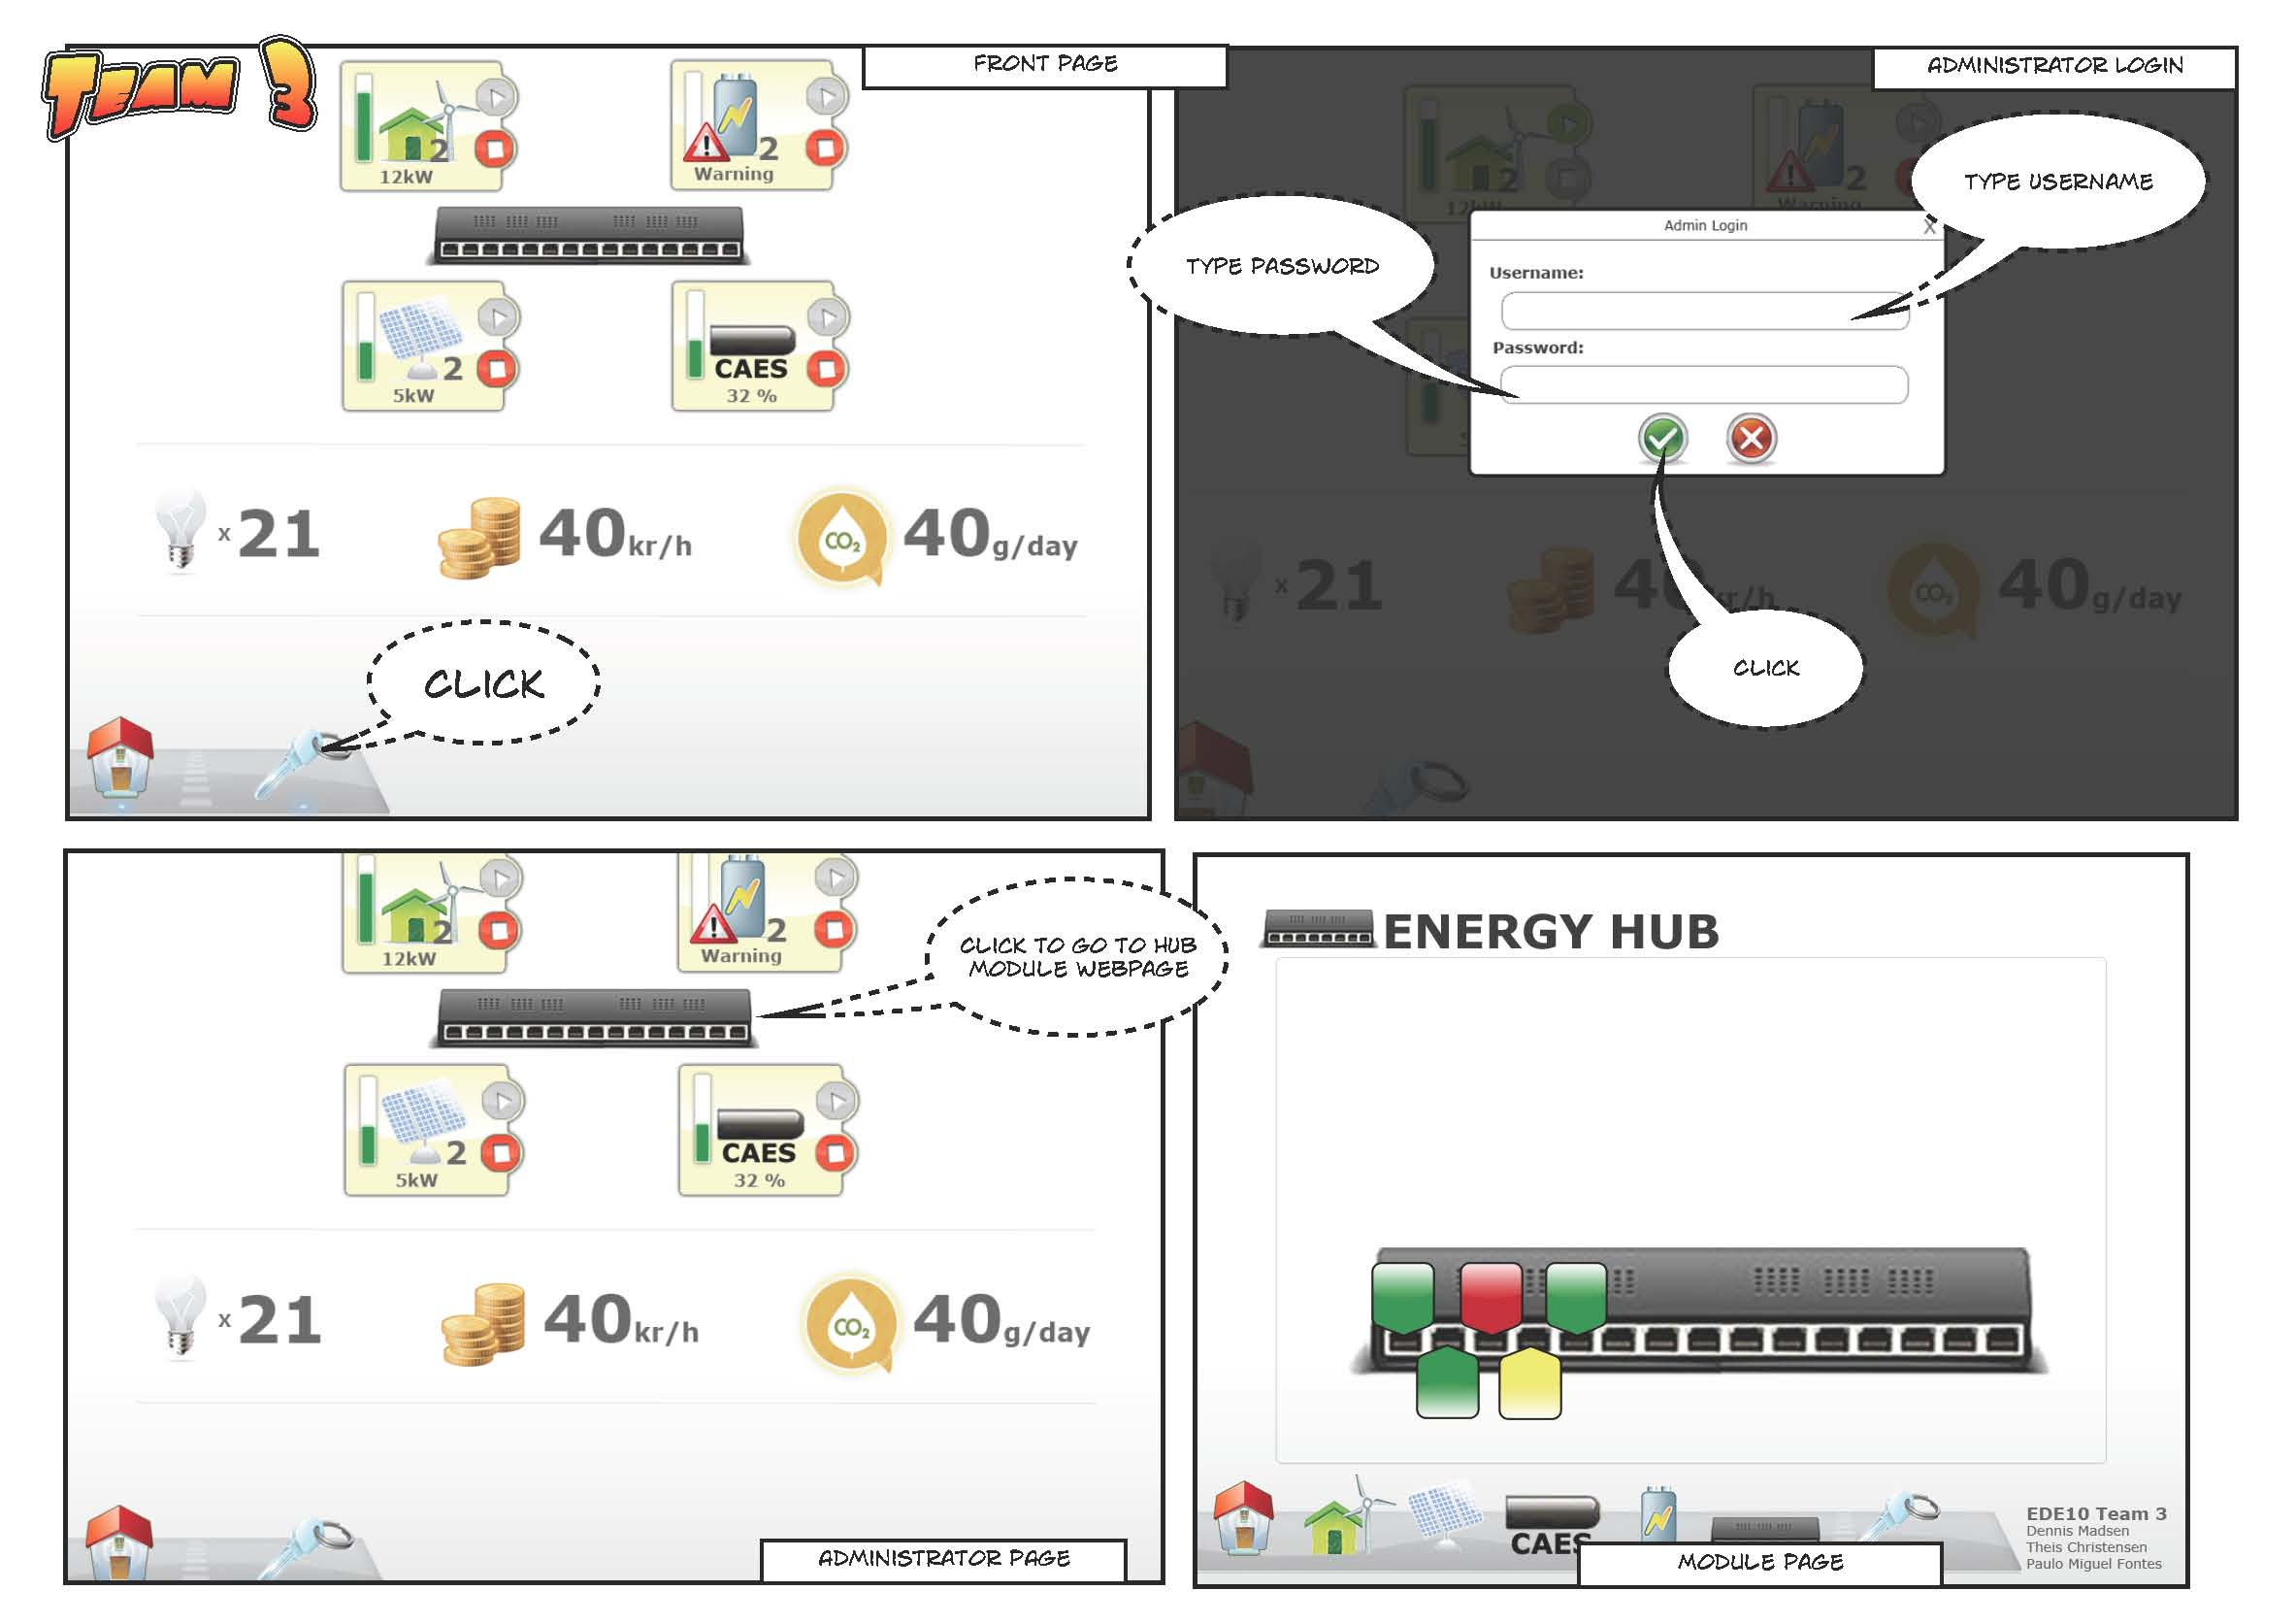
\includegraphics[width=0.4\textwidth]{images/web_interface1.jpg}}
   	\caption{Picture of the hub LF before session}
   	\label{fig:LF hub before session}
\end{figure}
\begin{figure}[h!]
	\center
		\setlength\fboxsep{0pt}
		\setlength\fboxrule{1pt}
		\fbox{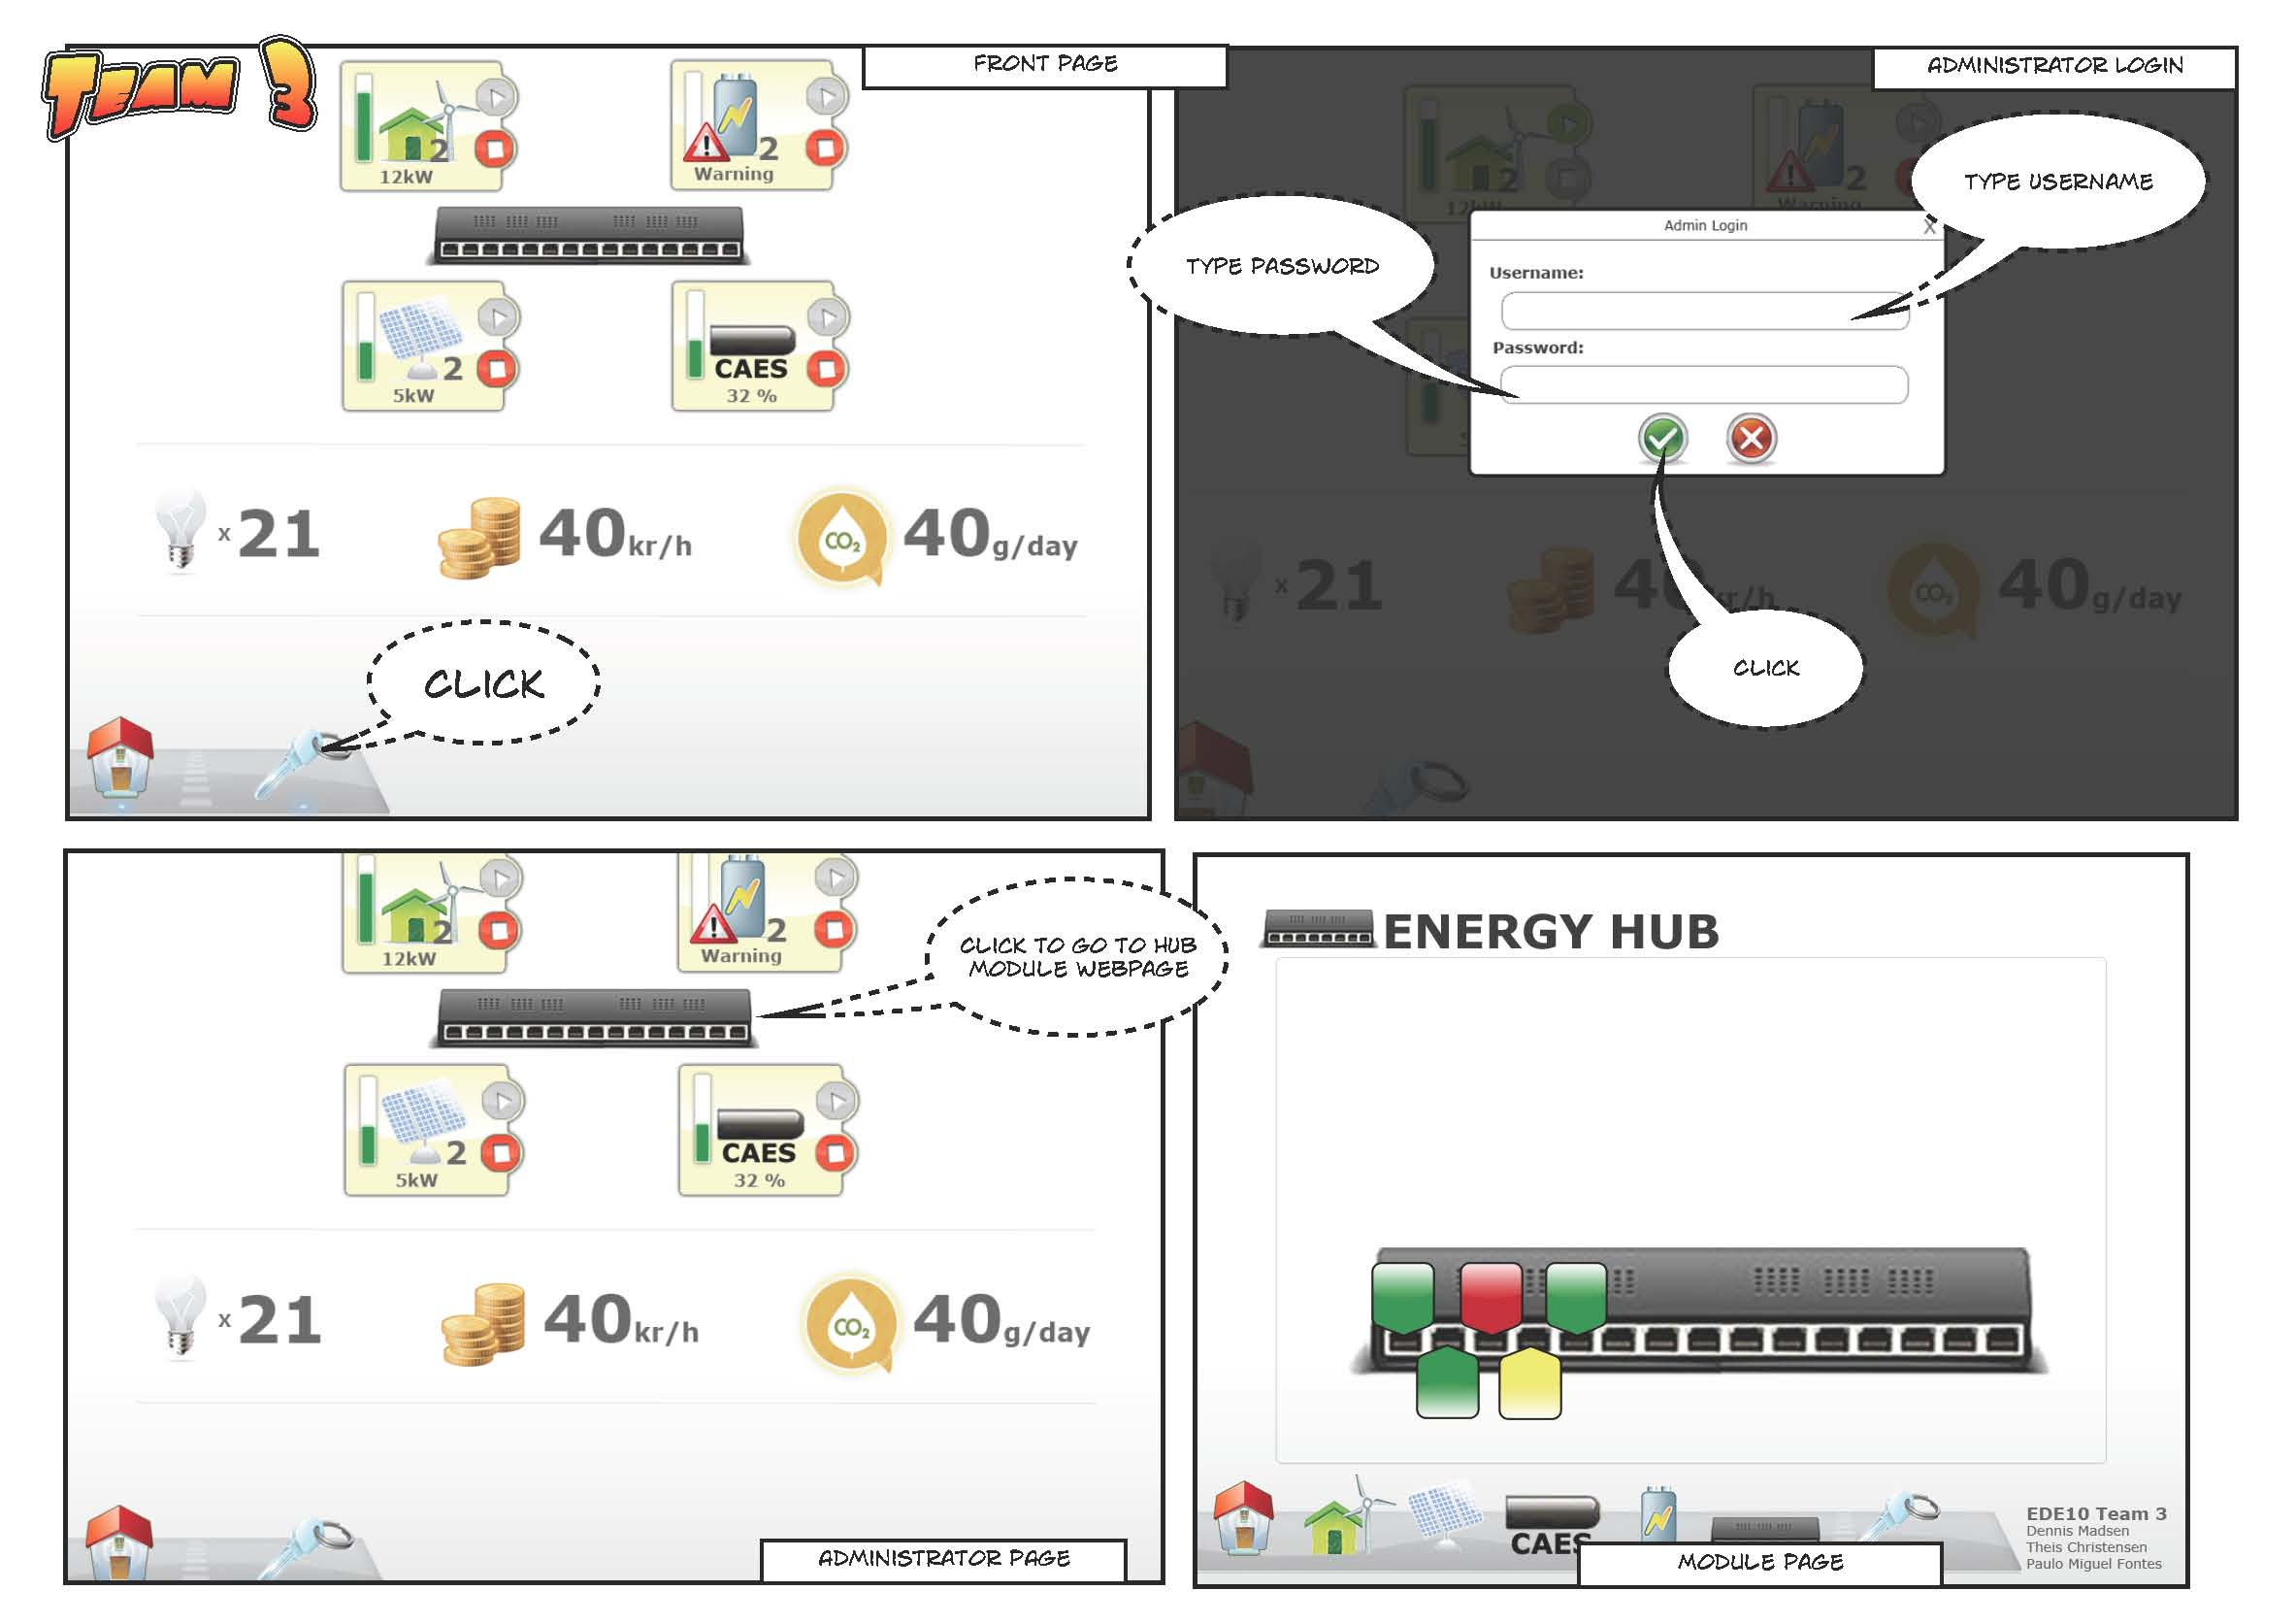
\includegraphics[width=0.4\textwidth]{images/web_interface1.jpg}}
   	\caption{Picture of the hub LF after session}
   	\label{fig:LF hub after session}
\end{figure}

\subsection{Hub high fidelity}
The high fidelity hub prototype was made before we had the participatory design session. This was how we have defined his needs, and how we think it should looks like. The prototype is also used in the participatory design. We made it with the same box as the low fidelity hub prototype, we used a mbed to control the LEDs and bottoms in the front sheet. This is a high fidelity prototype, because it can show how the hub will react on different actions, it gives the user the same experience as a fully operational hub would with this user interface.
\begin{figure}[h!]
	\center
		\setlength\fboxsep{0pt}
		\setlength\fboxrule{1pt}
		\fbox{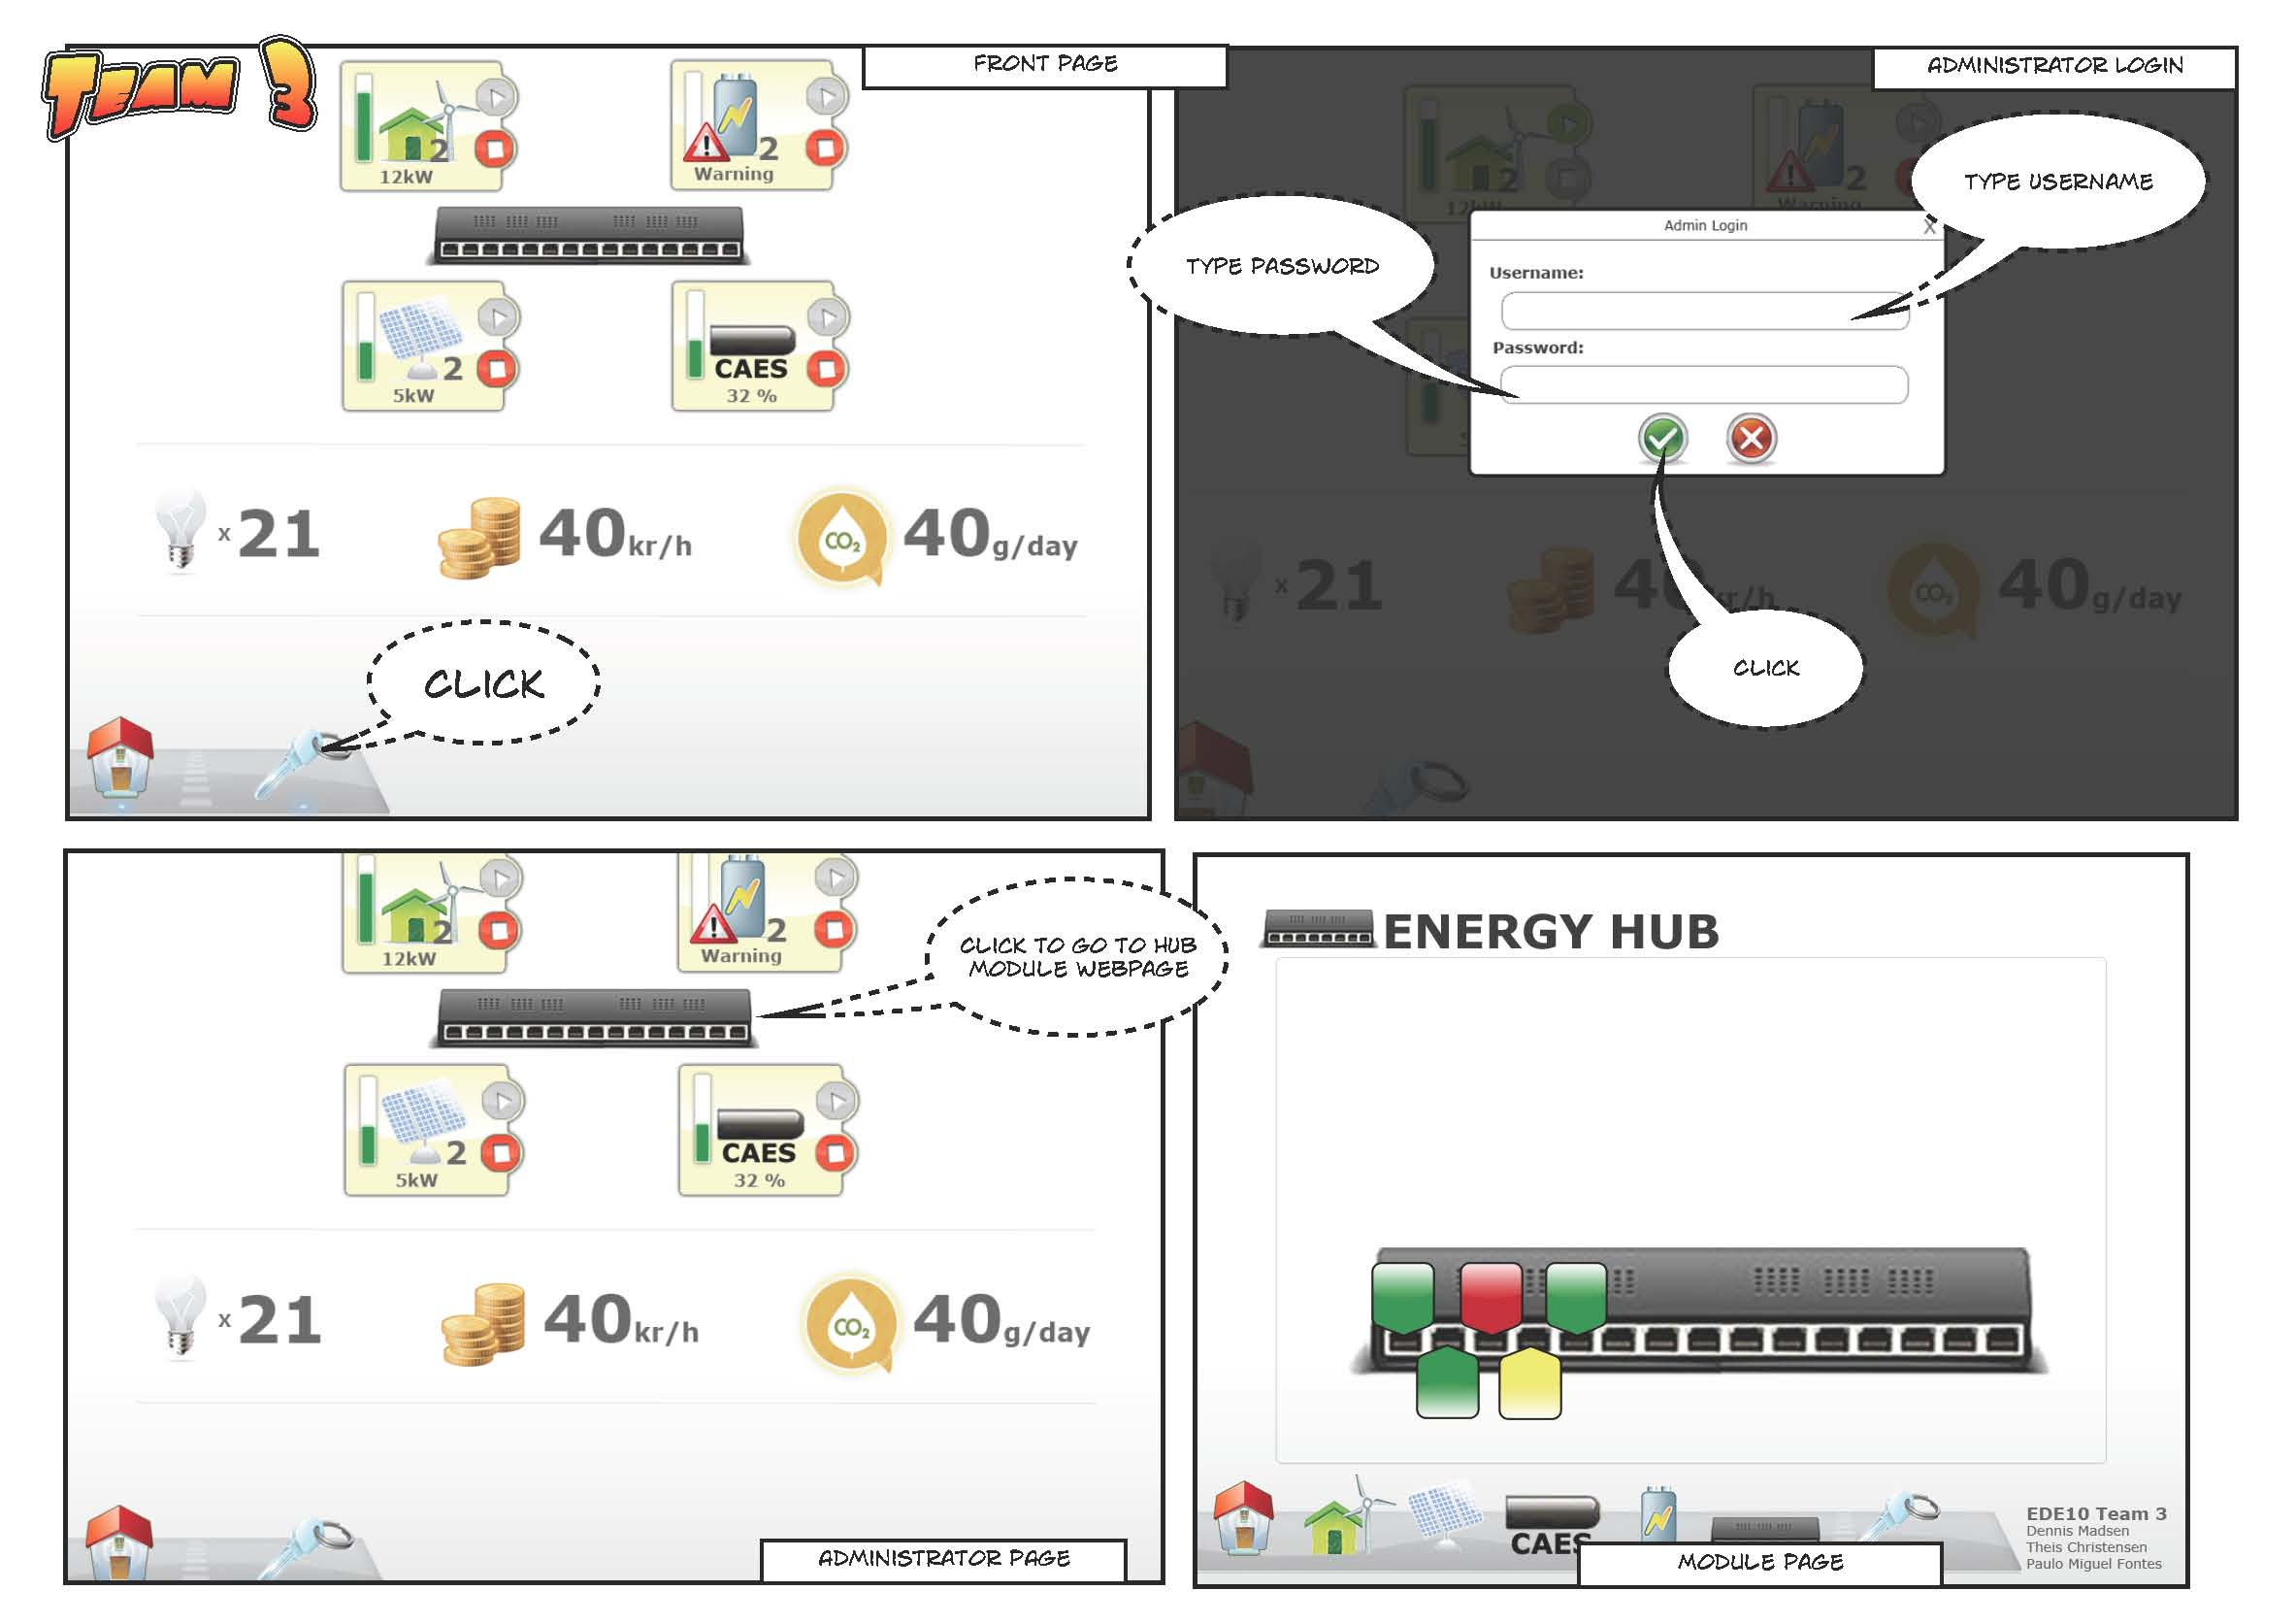
\includegraphics[width=0.4\textwidth]{images/web_interface1.jpg}}
   	\caption{Picture of the hub HF}
   	\label{fig:High fidelity hub}
\end{figure}

\subsection{Power point mid fidelity}
The power point prototype is used in the first usability test. It is an interactive power point with slides to show the different web pages, we have said that this is a mid fidelity prototype, it gives the user a good experience as the final page would do, but it dose not have any dynamic data, it is all static so that it is just to see how the interaction with the page works.
\begin{figure}[h!]
	\center
		\setlength\fboxsep{0pt}
		\setlength\fboxrule{1pt}
		\fbox{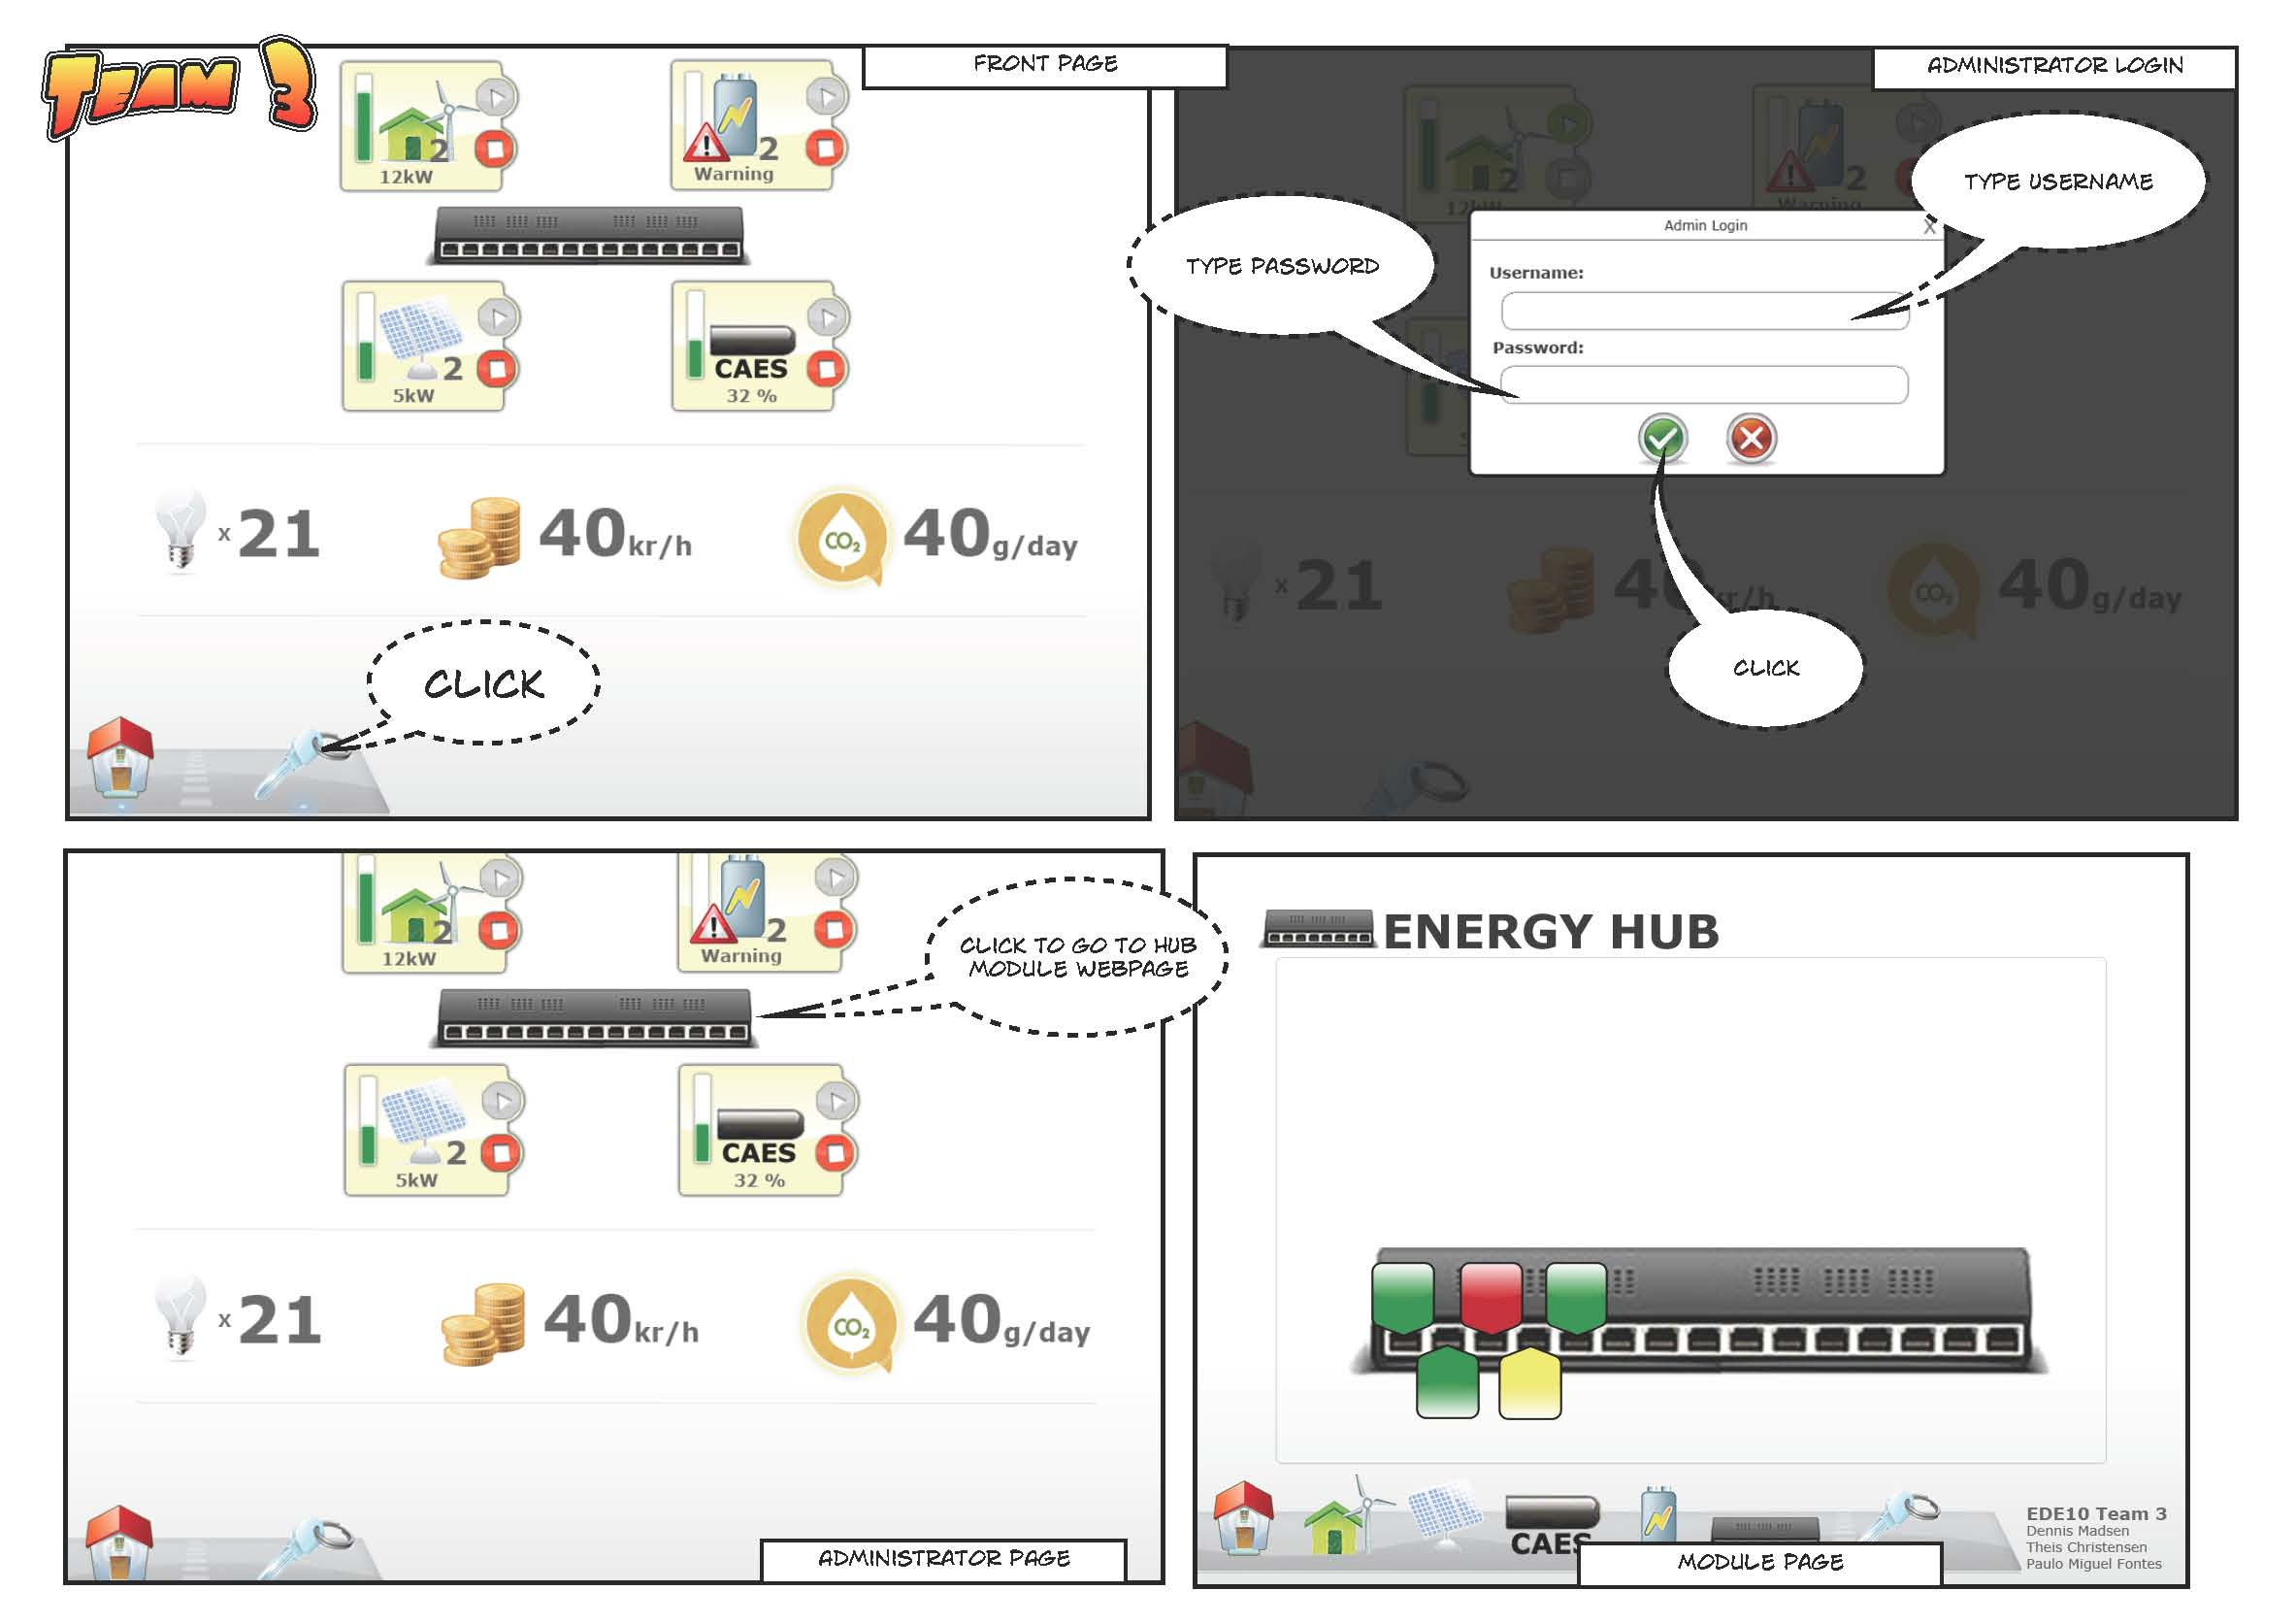
\includegraphics[width=0.4\textwidth]{images/web_interface1.jpg}}
   	\caption{Picture of the power point slides}
   	\label{fig:web_interface1}
\end{figure}

\subsection{HTML web page mid fidelity}
The HTML page prototype is used in the second usability test. It is the web page developed in EWEB1 course, the purpose of the site is to give at picture of how the final web page would look like and work but without any data reading and logging, it is a static web page. We had said this to be mid fidelity as the power point because it perform the same purpose and have the same functionality.
\begin{figure}[h!]
	\center
		\setlength\fboxsep{0pt}
		\setlength\fboxrule{1pt}
		\fbox{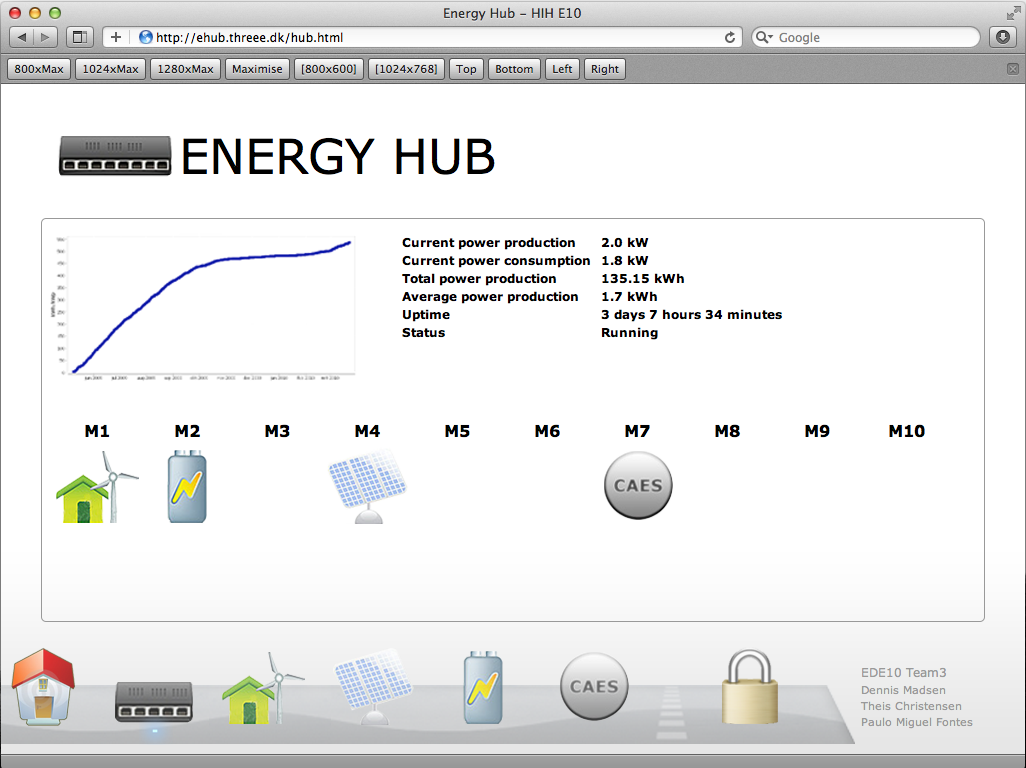
\includegraphics[width=0.4\textwidth]{images/screen_hub_page.png}}
   	\caption{Picture of the hub web page}
   	\label{fig:web_hub_interface}
\end{figure}
\begin{figure}[h!]
	\center
		\setlength\fboxsep{0pt}
		\setlength\fboxrule{1pt}
		\fbox{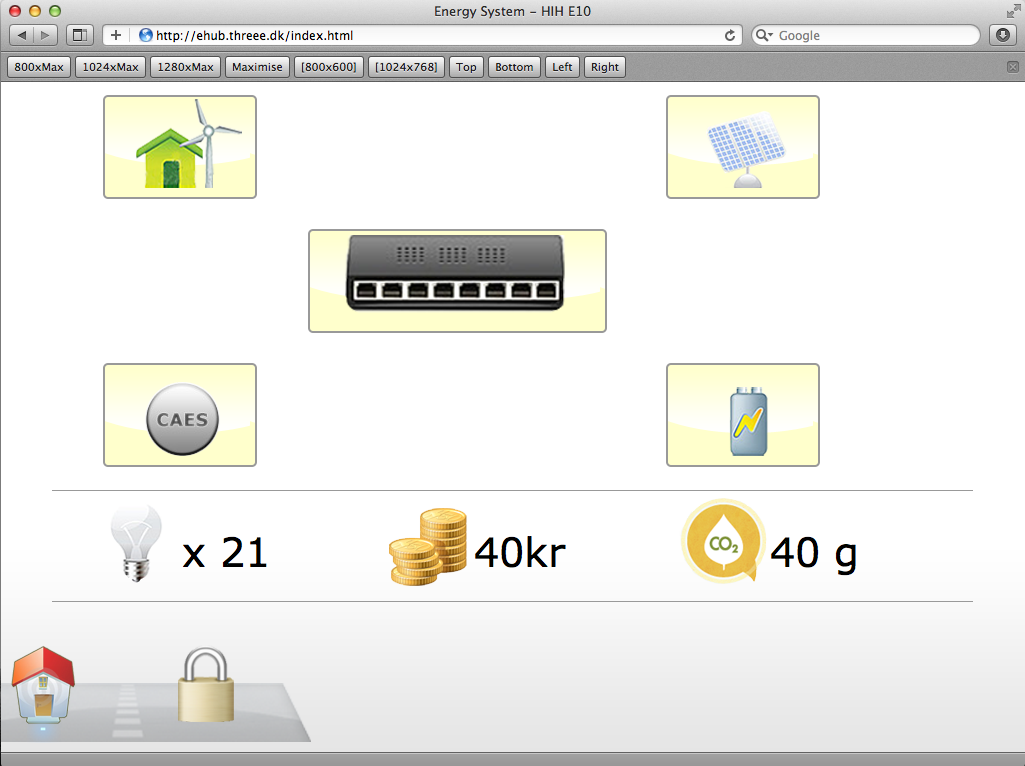
\includegraphics[width=0.4\textwidth]{images/screen_index_page.png}}
   	\caption{Picture of the index web page}
   	\label{fig:web_index_interface}
\end{figure}%%%%%%%%%%%%%%%%%%%%%%%%%%%%%%%%%%%%%%%%%
\section{Participatory Design - Dennis}
As explained earlier, the hub module is divided into two sections, the web interface and the physical interface on the hub. 
The goal of the participatory design session with the customer Jan was to clarify the level of interaction he wants on the hub module, but also where the different things should be placed. A video of the session can be found on the wiki page (find link in the introduction section). Before the session, pictures of small buttons, LED's, screens, connecters etc. were printed out to easy to process of placing components on the front panel. Jan's job was now, with some guidance instructions, to place the components he wanted on the hub and where he wanted them. The design ended up with a clean design containing: 
\begin{itemize}
	\item 1 Power button, to turn on the hub. The button should have built in LED.
	\item 1 emergency button (powers off everything).
	\item 1 on/off switch for each module (position switch).
	\item 2 indication LED for each module (green on = module is powered on. Red on = module is powered off).
	\item A 230VAC plug is placed on the front to connect: light, phone-chargers or similar. 
\end{itemize}
To get access to the front panel of the hub, a locker should be open with a key, to protect agains fiddle-fingers. The emergency button is of cause operational all the time, and no locker needs to be opened to use it.
\\When finishing his idea about the front panel of the hub, Jan was introduced to another solution, which worked as a prototype of the finish product. Jan was asked to go through some tasks:
\begin{itemize}
	\item Turn on the hub.
	\item Connect a module.
	\item Turn on the connected module.
	\item Identify an error on a module.
	\item Repair the module.
	\item Shut down the system.
\end{itemize}
The general impression from Jan was positive, but some of functions found on the interface was unnecessary as he will primarily use a PC to check the status of the different devices (on the web interface). The placement and method of connecting new devices was fine and the same with turning on and off the hub. Instead of the pushbuttons found on the prototype, as mentioned, he wants position switches. The indication of every module was fine, but unnecessary indicators should be removed. 
%%%%%%%%%%%%%%%%%%%%%%%%%%%%%%%%%%%%%%%%%
\section{First usability tests - Theis}
In the first usability test we used the power point as a demonstration prototype of the web page. We made two sessions, one with Rene and one with Jan as the web customer and the full system customer. We had a camera, to record the actions on the screen, and another to record the face expressions. In the sessions Rene and Jan had free hands to play around with the power point. The goal of this test was most of all to show the design we had made, and then get some reactions and comment on what was good and what was bad. There was no specific tasks that the users should do, so this was not completely a usability test. Both Rene and Jan was positive surprised, but they had also a lots of things that they would have on the final page.\\\\
\textbf{Rene would like:}
\begin{itemize}
	\item Identify modules - Give an ID for each modules so they can be identified easily
	\item Warnings - Optimise warning status for a more intuitive experience (maybe change background of the icon)
	\item Graphs - Make the graphs full screen when click on
	\item Permissions - User without log in should be allow to see everything but not change it
	\item Status - Make vertical bar more intuitive, add colour scheme to it (red, yellow, green)
	\item Update - The data should update every 5 to 10 seconds
\end{itemize}
\textbf{Jan would like:}
\begin{itemize}
	\item Small data font - Make bigger data text
	\item Explanation for graphs - Make a small explanation for what the graphs shows
	\item Graphs - Make the graphs full screen when click on
	\item Energy for storage device - Show the energy for storage modules for comparing with other modules
	\item Start/Stop - The start and stop function for the modules did not work intuitive for him
	\item Not exciting - The page was a bit boring
\end{itemize}
In the development of the final web page, with all the PHP and dynamic integration, we will consider every suggestion from the two sessions. Identifying the modules will be taken care of with the PHP, so when you click the wind turbine and there is more than one of them every module will be shown with there ID so the user easily can figure out what module he wants to look at. The warnings should be more visible, Rene suggested to maybe change the background color of the module when there is an error. This observation got a supported very well in the session with Jan, he did not notice that there was an error on one of the batteries, we will make the warnings more visible on the final page, and maybe use the suggestion from Rene with the background color. Both Jan and Rene wanted to make the graphs full screen when they click on them, this will also be implemented in the final page, maybe with a page where the user can change settings for the graphs and see explanation for what the graph shows. The permissions for users without log in, is already implemented in the HTML page. The both wanted more data on the modules, and comparison options between the modules and the specification of the modules, this will be implemented on the final page, when it is possible to get all data through PHP implementation. Rene wanted the data to update every 5 to 10 seconds, this would be waste of resources if no one is looking at the web interface, to optimize this, the web interface would check if anyone is using the page, if someone is using i the data will be updated from the log every 5 - 10 seconds. Jan said that the font was a bit small, this will be helped so it is easy to change the text size on the page. Jan also said that the page was not exciting, and suggested to use more color, but we think it is because of the page is static, in the final page there will be used java scripting to make effect and animation on the page, we think that will help on the excitement for the web page. Jan did not think out start and stop bottoms was intuitive, because of the colors and there was no clearly status indication of the single module, this will be made with a status box for each module clearly showing the status of the module.


%%%%%%%%%%%%%%%%%%%%%%%%%%%%%%%%%%%%%%%%%
\section{Second usability tests - Paulo}

In this usability test, tasks were defined and asked for the users to follow. Users were timed for each task, is important to know how much time users will take to do each task so we can understand the difficulty of the navigation in our interface and what could be change to make it more understandable for the user.
\\
\\Three different individual where selected to this usability test:\\
- Person directly involved on the project.\\
- Person with an overview of the project.\\
- Person without not involved, or overview of the project.\\
\\
5 tasks were asked to the users:\\
- Login as an admin user.\\
- View photovoltaic page.
- See the average power on the energy hub.\\
- Find the current status on the battery module.\\
- Log out.
\\















